\section{Breve descrizione dell'implementazione del firmware originale}

\begin{frame}{Introduzione}
  In questa sezione vengono illustrate le principali funzioni e strutture dati
  del firmware che implementano il sistema descritto.\\
  Per una descrizione più approfondita si rimanda ai diagrammi allegati con il presente
  report contenenti
  \begin{itemize}
  \item[-] la macchina a stati dal punto di vista di un tag;
  \item[-] la macchina a stati dal punto di vista di un'ancora;
  \item[-] un sequence diagram che descrive la procedura di ranging;
  \item[-] un sequence diagram che descrive la ``nuova'' procedura di autoranging
    (descritta nel seguito).
  \end{itemize}
\end{frame}

\begin{frame}{Struttura cartelle firmware}
  \begin{columns}
    \begin{column}{0.6\textwidth}
      Le cartelle contententi i file più imporanti del firmware sono indicate nella figura a lato\\
      \begin{itemize}
      \item[-] \lstinline!instance.c! contiene la macchina a stati principale del sistema;
      \item[-] \lstinline!instance_common.c! contiene le \alert{callback} di ricezione e trasmissione;
      \item[-] \lstinline!main.c! contiene diverse strutture dati di interesse.
      \end{itemize}
    \end{column}
    \begin{column}{0.3\textwidth}
      \centering
      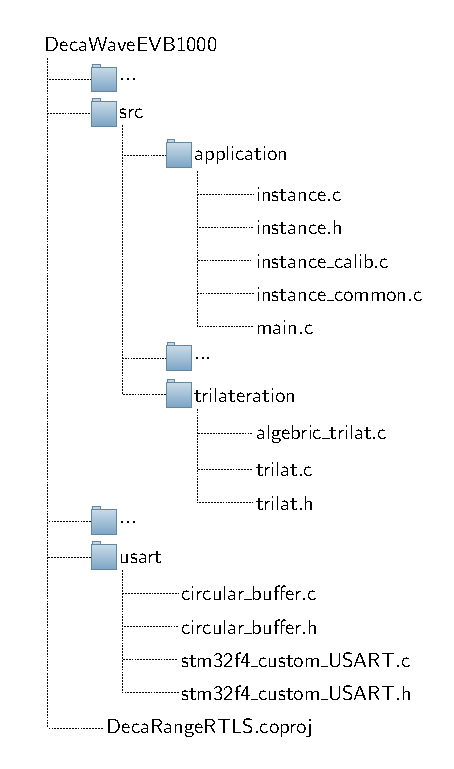
\includegraphics[height=20em]{file_tree_original.pdf}
    \end{column}
  \end{columns}
\end{frame}

\begin{frame}[fragile, shrink=20]{File \lstinline!main.c! - \lstinline!sfConfig!}
  Il file \lstinline!main.c! contiene, tra le altre cose, la \lstinline!struct sfConfig!
  che definisce la durata del frame e del superframe.\\
  Nel caso in cui gli switch sul PCB siano configurati per la modalità di trasmissione
  $6.8$mbps e canale $5$ la parte di interesse è quella che segue il commento
  \lstinline!//mode 2 - S1: 2 on, 3 off!
  \begin{C}
      sfConfig_t sfConfig[4] =
      {
      ...
      //mode 2 - S1: 2 on, 3 off
      {
        (10),    // durata del frame in ms
        (10),    // numero di slot
        (10*10), // durata superframe (T_sf)
        (10*10), // periodo ideale attivazione del tag (T_sp)
        (2500)   // delay di trasmissione del Final (T_fd)
      },
      ...
    };
\end{C}
  La modifica di questi parametri consente di cambiare la frequenza di funzionamento
  del sistema e il numero massimo di tag supportati.
\end{frame}

\begin{frame}{File \lstinline!instance.c! - Macchina a stati}
  Il file \lstinline!instance.c! contiene, tra le altre cose, la funzione
  \lstinline[language=C]!int testapprun(instance_data_t *inst, ...)!
  che implementa la macchina a stati del sistema.\\
  Il puntatore \lstinline!inst! contiene l'indirizzo di un'istanza della struttura
pp  \lstinline!instance_data_t!, definita in \lstinline!instance.h!, che contiene
  principalmente lo stato della macchina a stati.\\
  Di seguito vengono brevemente descritti gli stati. Per ulteriori dettagli si rimanda
  ai diagrammi allegati con il presente report.
  \begin{itemize}
  \item[-] \lstinline!TA_INIT!: stato nel quale il dispositivo viene inizializzato;
  \item[-] \lstinline!TA_RXE_WAIT! : stato di transizione verso lo stato \lstinline!TA_RX_WAIT_DATA!;
  \item[-] \lstinline!TA_RX_WAIT_DATA! : stato nel quale il dispositivo attende e processa i messaggi ricevuti dal tag o dalle ancore a seconda della loro tipologia;
  \end{itemize}
\end{frame}

\begin{frame}{File \lstinline!instance.c! - Macchina a stati}
  \begin{itemize}
  \item[-] \lstinline!TA_TXE_WAIT!: stato nel quale il tag valuta i range numerici a partire dai tempi di volo ottenuti dalle ancore nell'ultima istanza di ranging;
  \item[-] \lstinline!TA_SLEEP_DONE!: stato nel quale il tag attende l'arrivo del successivo istante di invio Poll;
  \item[-] \lstinline!TA_TXPOLL_WAIT_SEND!: stato in cui viene inviato il Poll;
  \item[-] \lstinline!TA_TX_WAIT_CONF!: stato in cui viene calcolato il Final Delay $T_{fd}$ (vedi slide \ref{delayed_tx})
    ossia l'istante (RMARKER) in cui dovrà essere spedito il Final;
  \item[-] \lstinline!TA_TX_FINAL_WAIT_SEND!: stato in cui si spedisce il messaggio di Final.
  \end{itemize}
\end{frame}

\begin{frame}[shrink=20]{Stato \lstinline!TA_RX_WAIT_DATA! - Tipologia dei messaggi}
  Lo stato \lstinline!TA_RX_WAIT_DATA! processa i messaggi ricevuti a seconda della tipologia degli stessi.
  La tipologia è indicata dal primo byte del campo \lstinline!msg_data! e sarà indicato nel seguito come \lstinline!FCODE!.
  \begin{center}
    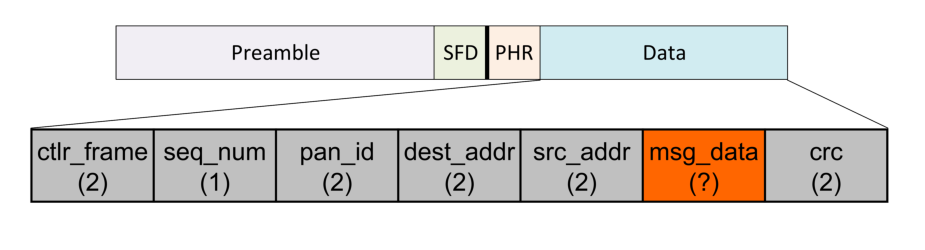
\includegraphics[height=10em]{whole_msg_with_payload}
  \end{center}
  Gli \lstinline!FCODE! possibili nella implementazione originale sono
  \begin{itemize}
  \item[-] \lstinline!RTLS_DEMO_MSG_TAG_POLL!: identifica un messaggio di Poll inviato da un tag;
  \item[-] \lstinline!RTLS_DEMO_MSG_TAG_FINAL!: identifca un messaggio di Final inviato da un tag;
  \item[-] \lstinline!RTLS_DEMO_MSG_ANCH_RESP!: identifica un messaggio di Risposta ad un Poll inviato da un'ancora.
  \end{itemize}
\end{frame}

\begin{frame}[fragile]{File \lstinline!instance_common.c! - Callback di trasmissione}
  Ogni volta che viene inviato un messaggio attraverso il circuito DecaWave DWM1000
  lo stesso si preoccupa di interrompere il microcontrollore del DecaWave EVB1000 per segnalare
  l'esito dell'invio del messaggio. L'interruzione determina l'esecuzione della funzione
  \begin{C}
    instance_txcallback(const dwt_callback_data_t *txd)
  \end{C}
  Quando viene eseguita tale funzione all'indirizzo memorizzato in \lstinline!txd! è stato già
  salvato l'esito della trasmissione (che è stato trasferito tramite SPI).\\
  Generalmente l'esito della trasmissione viene acceduto all'interno della macchina a stati
  nello stato \lstinline!TA_TX_WAIT_CONF!.
\end{frame}

\begin{frame}[fragile]{File \lstinline!instance_common.c! - Callback di ricezione}
  La macchina a stati è inoltre \alert{affiancata} da un meccanismo basato su callback per la ricezione dei messaggi.
  Ciò significa che ogni volta che il circuito integrato DecaWave DWM1000 riceve un messaggio
  interrompe il microcontrollore del DecaWave EVB1000 determinando l'esecuzione della funzione
  \begin{C}
    instance_rxcallback(const dwt_callback_data_t *rxd)
  \end{C}
  Quando viene eseguita tale funzione all'indirizzo memorizzato in \lstinline!rxd! è stato già
  salvato il messaggio ricevuto (che è stato trasferito tramite SPI).
\end{frame}

\begin{frame}[shrink=10, fragile]{File \lstinline!instance_common.c! - Callback di ricezione}
  A seconda dell'\lstinline!FCODE! del messaggio la callback di ricezione determina un comportamento diverso
  del tag o dell'ancora.
  Principalmente 
  \begin{itemize}
  \item[-]un'ancora che riceve un \lstinline!RTLS_DEMO_MSG_TAG_POLL! prepara il messaggio di Risposta e se è il suo turno
    invia il messaggio di Risposta; 
  \item[-]un tag che riceve un \lstinline!RTLS_DEMO_MSG_ANCH_RESP! memorizza l'RMARKER di ricezione della risposta nel campo dati
    del prossimo messaggio di Final. Se deve attendere altre risposte resta in modalità di ricezione. Diversamente si prepara ad inviare
    il Final;
  \item[-]un'ancora che riceve un \lstinline!RTLS_DEMO_MSG_ANCH_RESP! aggiorna il contatore \lstinline!responeTO! che contiene il numero
    di risposte che l'ancora si aspetta ancora di ricevere (vedi slide \ref{anchors_responses_turn}). Se è il suo turno invia il messaggio di Riposta;
  \item[-]un'ancora che riceve un \lstinline!RTLS_DEMO_MSG_TAG_FINAL! si prepara al calcolo del ToF che avverrà nella macchina a stati.
  \end{itemize}
\end{frame}

\begin{frame}{Struttura generale di un messaggio}
  Di seguita si riporta la struttura del campo Data di un messaggio generico.
  \begin{center}
    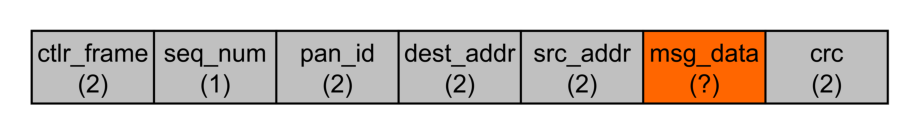
\includegraphics[height=3.4em]{message_f.pdf}
  \end{center}
  \vskip-2em
  \begin{itemize}
  \item[-] \lstinline!ctrl_frame!: maschera nella quale, tra le varie cose, viene decisa la modalità di
    indirizzamento
  \item[-] \lstinline!seq_num!: sequence number
  \item[-] \lstinline!pan_id!: ID della rete
  \item[-] \lstinline!dest_addr!: indirizzo del destinatario
  \item[-] \lstinline!src_addr!: indirizzo del mittente
  \item[-] \lstinline!msg_data!: payload (dipende dal tipo di messaggio)
  \item[-] \lstinline!crc!: cyclic redundandcy check
  \end{itemize}
  Nelle slide successive viene riportata la struttura del campo \lstinline!msg_data! per gli \lstinline!FCODE! descritti precedentemente.
\end{frame}

\begin{frame}{Messaggio di Poll - \lstinline!RTLS_DEMO_MSG_TAG_POLL!}
  \begin{center}
    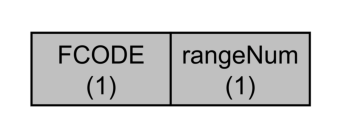
\includegraphics[height=3.4em]{message_f_tag_poll.pdf}
  \end{center}
  \begin{itemize}
  \item[-] \lstinline!FCODE = RTLS_DEMO_MSG_TAG_POLL!
  \item[-] \lstinline!rangeNum!: range number della trasmissione
  \end{itemize}
\end{frame}

\begin{frame}{Messaggio di Final - \lstinline!RTLS_DEMO_MSG_TAG_FINAL!}
  \begin{center}
    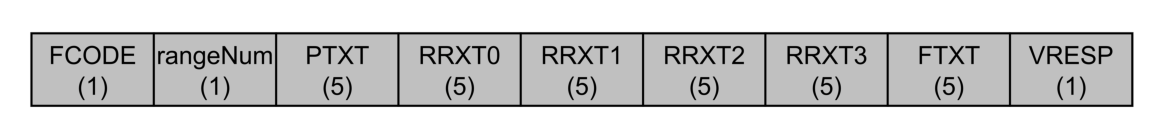
\includegraphics[height=3.4em]{message_f_tag_final.pdf}
  \end{center}
  \begin{itemize}
  \item[-] \lstinline!FCODE = RTLS_DEMO_MSG_TAG_FINAL!
  \item[-] \lstinline!rangeNum!: range number della trasmissione
  \item[-] \lstinline!PTXT!: tempo di invio del Poll
  \item[-] \lstinline!RRXT0!: tempo di ricezione della risposta da ancora 0
  \item[-] \lstinline!RRXT1!: tempo di ricezione della risposta da ancora 1
  \item[-] \lstinline!RRXT2!: tempo di ricezione della risposta da ancora 2
  \item[-] \lstinline!RRXT3!: tempo di ricezione della risposta da ancora 3
  \item[-] \lstinline!FTXT!: tempo di invio del Final
  \item[-] \lstinline!VRESP!: maschera della risposte valide ricevute
  \end{itemize}
\end{frame}

\begin{frame}{Messaggio di Risposta - \lstinline!RTLS_DEMO_MSG_ANCH_RESP!}
  \begin{center}
    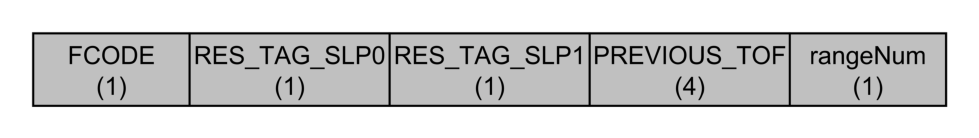
\includegraphics[height=3.4em]{message_f_anch_resp.pdf}
  \end{center}
  \begin{itemize}
  \item[-] \lstinline!FCODE = RTLS_DEMO_MSG_ANCH_RESP!
  \item[-] \lstinline!RES_TAG_SLP0!: parte alta dello sleep correction calcolato dall'ancora 0
  \item[-] \lstinline!RES_TAG_SLP1!: parte bassa dello sleep correction calcolato dall'ancora 0
  \item[-] \lstinline!PREVIOUS_TOF!: tof calcolato al passo precedente dall'ancora
  \item[-] \lstinline!rangeNum!: range number della trasmissione
  \end{itemize}
\end{frame}

